\section{Fourierreihe}
Die Fourierreihe $FR$ von einer Funktion $f(t)$ besteht aus Fourierkoeffizienten und entsprechender Basis in unendlich vielen Dimensionen:
\[
FR[f(t)] = \frac{a_0}{2} + \sum_{n = 1}^{\infty}[a_n \cdot \cos(n\omega_ft) + b_n \cdot \sin(n\omega_ft)]
\]

\noindent Dabei gilt, dass $\omega = \frac{2\pi}{T}$.

\noindent\textbf{Hinweis:} Immer zuerst überprüfen, ob eine Ähnliche $FR$ bereits existiert und mit Hilfe der Tip's in \ref{tip} berechnen.

\subsection{Fourierkoeffizienten}
Eine periodische Funktion $f$ mit \textbf{Periodendauer} $T > 0$, lässt sich durch eine Reihe von Sinus- und Kosinusfunktionen darstellen, deren Frequenzen ganzzahlige Vielfache der Grundfrequenz $\omega = 2\pi/T$ sind:
\[f(t) = \frac{a_0}{2} + \sum_{n = 1}^{\infty}[a_n \cdot \cos(n\omega_ft) + b_n \cdot \sin(n\omega_ft)]\]
\subsubsection{$\mathbb{R}$ Koeffiziente}
\noindent Konkret können die Koeffizienten der Funktion $f(t)$ folgendermassen berechnet werden ($n \in [1;\infty]$):
\[
a_n = \frac{2}{T}\int_{0}^{T}f(t) \cdot \cos(n\omega t)dt \qquad b_n = \frac{2}{T}\int_{0}^{T}f(t) \cdot \sin(n\omega t)dt
\]

\noindent Der erste Koeffizient $a_0 = \frac{1}{T}\int\limits_{0}^{T}f(t)dt$ der Funktion $f(t)$ ist der Mittelwert im Intervall $(0; T)$. Bei einer \underline{Fallunterscheidung} von $f(t)$ müssen Integrale von allen Fällen (mit entsprechenden Grenzen von $f_n$) summiert werden.
~\\

\noindent\textbf{Hilfe:} $\cos(n\pi) = (-1)^n$ und $\sin(n\pi) = 0$ 
~\\

\subsubsection{$\mathbb{C}$ Koeffiziente}
\noindent Mittels der komplexen Darstellung werden die Fourierkoeffizienten mit $c_n \rightarrow \Re(c_n) = a_n; \Im(c_n) = b_n$ dargestellt.
\[
\sum_{n=-\infty}^{\infty}c_n \cdot e^{jk\omega t}
\]
Diese Fourierkoeffizienten $c_n$ können mit einer einzigen Integration berechnet werden:
\[
c_n = \frac{1}{T} \int_{0}^{T}f(t)\cdot e^{-jn\omega t} dt
\]

\noindent\textbf{Hilfe:} $e^{-jn\pi} = (-1)^n$ und $e^{-jn2\pi} = 1$

\subsubsection{Umrechnung}\label{umrechnung}
Um Komplexe zu Reellen Koeffizieten umzurechnen können folgende Formeln gebraucht werden:
\begin{align*}
	c_n = \overline{c_{-n}} &= \frac{a_n - jb_n}{2} &\qquad n \in (0,1,2, \cdots, b_0 = 0) \\
	a_n &= 2\Re(c_n) = c_n + c_{-n}  &\qquad n \in (0,1,2, \cdots) \\
	b_n &= -2\Im(c_n) = j(c_n + c_{-n}) &\qquad n \in (1,2, \cdots) \\
\end{align*}

\subsection{Tip's}\label{tip}
\subsubsection{Funktionen mit Fallunterscheidungen}
Falls eine Funktion mit Fallunterscheidung in eine Fourierreihe transformiert werden muss, muss von Rand-zu-Rand integriert werden.

\noindent\textbf{Beispiel:}
\[
f(t)= e^{-\left|t\right|} \qquad t \in [-\pi;\pi] \qquad T = 2\pi
\]
\begin{center}
	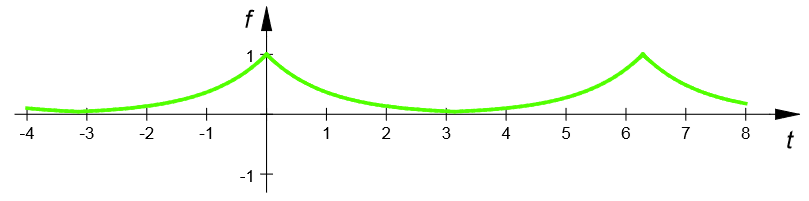
\includegraphics[width=0.6\columnwidth]{Images/beispiel_e_cn}
\end{center}

\noindent Dafür kann für Reelle Koeffizienten die Symmetrie ausgenutzt und von $[0;\pi]$ integriert werden. In der Komplexen Welt \textit{müssen} zwei Integrale berechnet werden:
\[
c_n = \frac{1}{2\pi}\int_{-\pi}^{0}e^t\cdot e^{-jnt}dt + \int_{0}^{\pi}e^{-t}\cdot e^{-jnt}dt
\]

\subsubsection{Symmetrie}
\textbf{ACHTUNG:} Gilt nur für $\mathbb{R}$ Fourierreihe! In $\mathbb{C}$ Reihe darf nicht über die halbe Periode Integriert und das Resultat verdoppelt werden! 
~\\
~\\
\noindent Für alle \textbf{geraden} (Achsensymmetrisch) T-periodische Funktionen ($f(t) = f(-t)$)  gilt $b_n = 0$ und für $a_n$ gilt: cos ist gerade 
\[
a_n = \frac{4}{T}\int_{0}^{\frac{T}{2}}f(t) \cdot \cos(n\omega t)dt
\]

\noindent Ist die Funktion \textbf{ungerade} (Punktsymmetrisch) ($f(-t) = -f(t)$) dann gilt $a_n = 0$ und für $b_n$: sin ist ungerade
\[
	b_n = \frac{4}{T}\int_{0}^{\frac{T}{2}}f(t) \cdot \sin(n\omega t)dt 
\]


\subsubsection{Linearität}
Wenn $f(t)$ und $g(t)$ zwei T-periodische Funktionen mit Fourierkoeffizienten $a_n^{(f)}$ und $b_n^{(f)}$ bzw.  $a_n^{(g)}$ und $b_n^{(g)}$ sind, dann hat die Funktion $h(t) = r \cdot f(t) + s \cdot g(t)$ mit festen $r,s \in \mathbb{R}$ folgende Koeffizienten:
\begin{align*}
	a_n^{(h)} &= r \cdot a_n^{(f)} + s \cdot a_n^{(g)} \\
	b_n^{(h)} &= r \cdot b_n^{(f)} + s \cdot b_n^{(g)} \\
\end{align*}
\noindent\textbf{Beispiel:}~\\
\noindent Funktion $g(t) = 1$ um einen Offset zu erzeugen. Dabei ist $s$ der Mittelwert von $h(t)$. Am Schluss gemäss Linearität alle neuen Koeffizienten berechnen.
\[
	s = \frac{1}{2} \qquad
	1 = r\cdot \frac{\pi}{4} + \frac{1}{2} \cdot 1 \Rightarrow r = \frac{2}{\pi}
\]
\begin{center}
	\includegraphics[width=0.7\columnwidth]{Images/linearität}
\end{center}

\subsubsection{Zeitstreckung/Stauchung}
Es sei $f$ eine T-periodische Funktion mit Fourierreihe und $g(t) = f(r \cdot t)$ mit $r \in \mathbb{R}\setminus0$.
\[
r = \begin{cases}
		r > 1, & \text{Stauchung}\\
		r < 1, & \text{Streckung}\\
		r < 0, & \text{Spiegelung inkl. Stauchung/Streckung}\\
	\end{cases}
\]

\noindent Dann gilt für die Fourierkoeffizienten:
\begin{align*}
	a_n^{(g)} &= a_n^{(f)} \\
	b_n^{(g)} &= \underbrace{\sgn(r)}_{\text{Vorzeichen von } r} \cdot b_n^{(f)} \\
\end{align*}

\noindent\textbf{ACHTUNG:} Die Fourierreihe $FR[f(t)]$ ändert, da die Periodendauer $T$ ändert. Das bedeutet neu ist $\omega_{\text{neu}} = \frac{2\pi}{T_{\text{neu}}}$. Beispiel für $T = 2 \rightarrow \omega_{\text{neu}} = \pi$:
\[
FR[f(t)] = a_0 + a_1\cdot\sin(1\pi t) + a_2\cdot\sin(2\pi t) + \cdots + a_n\cdot\sin(n\omega_{\text{neu}} t)
\]

\subsubsection{Zeitverschiebung}
Wenn eine Funktion $f(t)$ um $t_0$ verschoben wird $g(t) = f(t + t_0)$, gilt für die Fourierkoeffizienten von $g$.
\[
t_0 < 0 \Rightarrow \text{Links verschiebung} \qquad t_0 > 0 \Rightarrow \text{Rechts verschiebung}
\]

\noindent\textbf{Für $\mathbb{R}$}:
\begin{align*}
	a_n^{(g)} &= \cos(n\omega t_0) \cdot a_n^{(f)} + \sin(n\omega t_0) \cdot b_n^{(f)}  \\
	b_n^{(g)} &= -\sin(n\omega t_0) \cdot a_n^{(f)} + \cos(n\omega t_0) \cdot b_n^{(f)}  \\
\end{align*}

\noindent\textbf{Für $\mathbb{C}$}:
\[
c_n^{(g)} = e^{jn\omega t_0} \cdot c_n^{(f)}
\]

\subsection{Konvergenzverhalten}
Um das Konvergenzverhalten von $f$ und der Fourierreihe $\hat{f}$ zu untersuchen, wird die mittlere quadratische Abweichung verwendet:
\[
\Vert f - \hat{f} \Vert = \sqrt{\frac{2}{T}\int_{0}^{T}\left[f(t) - \hat{f}(t)\right]^2dt}
\]
\begin{center}
	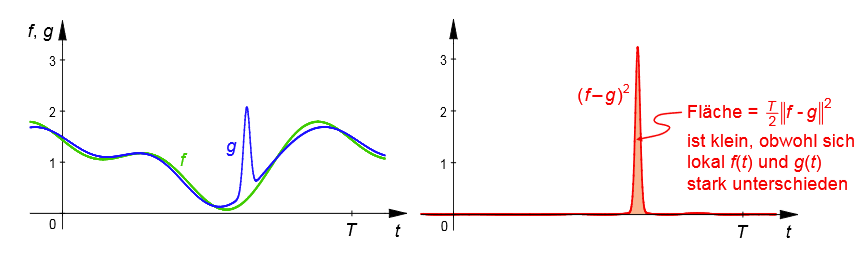
\includegraphics[width=\columnwidth]{Images/konvergenz}
\end{center}

\noindent Das hat zur Folge, dass die Fourierkoeffizienten $a_n$ und $b_n$ gegen $0$ konvergieren müssen. Je \textit{glatter} eine Funktion, desto schneller Konvergiert die Fourierreihe $\hat{f}$ mit der Original Reihe $f$. "Glat" bedeutet, je mehr Ableitungen ohne Sprungstellen oder Knicke eine Funktion $f^{(n)}$ hat, desto schneller konvergiert $f$.
~\\
\noindent Zudem gilt die Parseval'sche Gleichung:
\[
\frac{a_0^2}{2} + \sum\limits_{n=1}^{\infty}\left(a_n^2 + b_n^2\right) = \frac{2}{T}\int_{0}^{T}[f(t)]^2dt = \Vert f \Vert^2
\]
